\documentclass[10pt,table]{beamer}
\usepackage[utf8]{luainputenc}
\usepackage[ngerman]{babel}


%\usetheme[block=fill]{m}                     % Use metropolis theme
\usepackage{beamerthemeuzl-conference}

\usepackage{Alegreya,AlegreyaSans}

\logo{
\includegraphics[scale=.62]{uzl-logo-ITCS.pdf}}
\usepackage{amsmath}
\DeclareMathOperator*{\argmin}{arg\,min}
\usepackage{nicefrac}
\usepackage{algorithm}
\usepackage{dsfont}
\usepackage{subfig}
\usepackage{mathtools}
\usepackage{graphicx}
\usepackage{mathpazo} 
\usepackage{tikz}

\usepackage{algorithm}
\usepackage{algorithmic}
\usepackage{xspace}
\usepackage{float}
\usepackage{subfig}
\usepackage{color, colortbl}
\definecolor{uzlred}{HTML}{BF0000}
\definecolor{uzlgreen}{HTML}{008000}
\definecolor{uzlpurple}{HTML}{700080}
\newcommand{\highlightrow}{\rowcolor{Ozeangruen!5}}

\title{Algorithmen für das Moving-Target Travelling Salesman Problem}
%\subtitle{}
\author{Felix Greuling}
\date{27.01.2019}


\begin{document}
\maketitle


%\iffalse
\begin{frame}{Überblick}
\tableofcontents[hideallsubsections]
\end{frame}

\AtBeginSection[]
{
  \begin{frame}
    \frametitle{Überblick}
    \tableofcontents[currentsection, hideallsubsections]
  \end{frame}
}
%\fi

\AtBeginSection[]{
  \begin{frame}[noframenumbering]
  \vfill
  \centering
  \begin{beamercolorbox}[sep=8pt,center,shadow=true,rounded=true]{title}
    \usebeamerfont{title}\insertsectionhead\par%
  \end{beamercolorbox}
  \vfill
  \end{frame}
}



\section{Einleitung}
\begin{frame}{Einleitung}
Travelling Salesman Problem (TSP)
\begin{itemize}
\item
Optimierungsproblem aus der Kombinatorik
\item
Reihenfolge an Zielen, sodass die Tourzeit minimal ist
\item
Tour startet und endet im selben Ziel
\item
NP-vollständig
\end{itemize}
\end{frame}

\begin{frame}{Einleitung}
\begin{center}
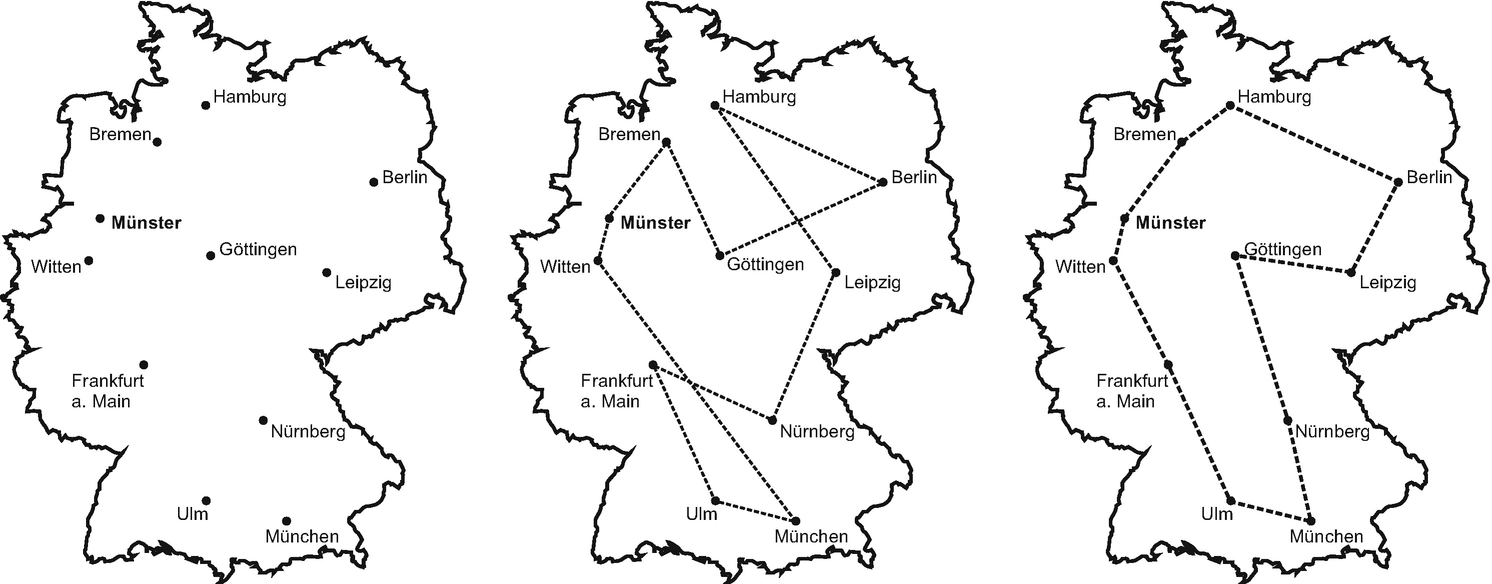
\includegraphics[scale=0.8]{Images/TSP.png}\\~\\
\small\cite{Grimme2018}
\end{center}
\end{frame}

\begin{frame}{Einleitung}
Moving-Target-TSP
\begin{itemize}
\item
Im Jahre 1998 von Helvig et al. erwähnt.
\item
Ziele sind nun nicht mehr stationär
\item
Problematik bleibt die selbe
\end{itemize}

\end{frame}

\begin{frame}{Einleitung}
\centering
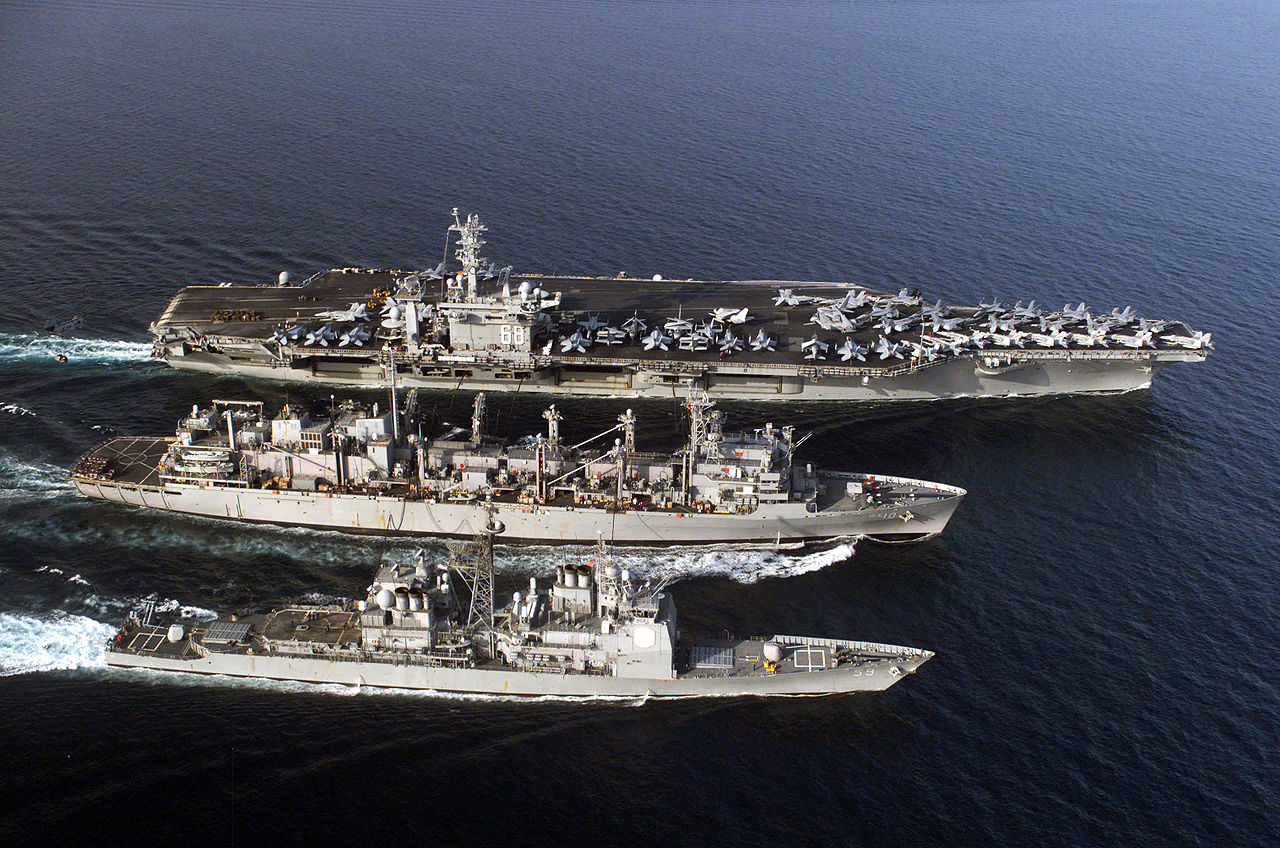
\includegraphics[scale=0.8]{Images/Versorgungsschiff.jpg}
%https://de.wikipedia.org/wiki/Versorgungsschiff#/media/Datei:USS_Nimitz_(CVN-68),_USS_Princeton_(CG-59)_and_USS_Bridge_(AOE-10).jpg
\end{frame}

\section{Grundlagen}
\begin{frame}{MT-TSP in einer Dimension}
Formal haben Helvig et al. das Problem wie folgt definiert \cite{helvig}:\\~\\
\begin{quote}
The moving-target traveling salesman problem: Given a set $S = \{s_1, \dots , s_n\}$ of \emph{targets}, each $s_i$ moving at constant velocity $\overrightarrow{v_i}$ from an initial position $p_i$, and given a \emph{pursuer} starting at the origin and having maximum speed $v>|\overrightarrow{v_i}|$, find the fastest tour starting (and ending) at the origin, which intercepts all targets.
\end{quote}
\end{frame}




\section{Zwei-orthogonale-Achsen im MT-TSP}

\subsection{Theoretische Grundlagen}

\subsection{Heuristiken}

\section{Ergebnisse}
\begin{frame}{Ergebnisse}

\end{frame}

\section{Zusammenfassung und Ausblick}
\begin{frame}{Zusammenfassung}
    
\end{frame}

\begin{frame}{Ausblick}

\end{frame}




\nocite{*}
\appendix
\begin{frame}[noframenumbering, plain]
\Large\center
Danke für Ihre Aufmerksamkeit!
\end{frame}


\begin{frame}[allowframebreaks, noframenumbering]{References} 
	\bibliographystyle{plain}
	\bibliography{lit}
\end{frame}

\end{document}
